\documentclass[journal,12pt,twocolumn]{IEEEtran}
\usepackage{setspace}
\usepackage{gensymb}
\usepackage{xcolor}
\usepackage{caption}
\singlespacing
\usepackage{siunitx}
\usepackage[cmex10]{amsmath}
\usepackage{mathtools}
\usepackage{hyperref}
\usepackage{amsthm}
\usepackage{mathrsfs}
\usepackage{txfonts}
\usepackage{stfloats}
\usepackage{cite}
\usepackage{cases}
\usepackage{subfig}
\usepackage{longtable}
\usepackage{multirow}
\usepackage{enumitem}
\usepackage{bm}
\usepackage{mathtools}
\usepackage{listings}
\usepackage{tikz}
\usetikzlibrary{shapes,arrows,positioning}
\usepackage{circuitikz}
\renewcommand{\vec}[1]{\boldsymbol{\mathbf{#1}}}
\DeclareMathOperator*{\Res}{Res}
\renewcommand\thesection{\arabic{section}}
\renewcommand\thesubsection{\thesection.\arabic{subsection}}
\renewcommand\thesubsubsection{\thesubsection.\arabic{subsubsection}}

\renewcommand\thesectiondis{\arabic{section}}
\renewcommand\thesubsectiondis{\thesectiondis.\arabic{subsection}}
\renewcommand\thesubsubsectiondis{\thesubsectiondis.\arabic{subsubsection}}
\hyphenation{op-tical net-works semi-conduc-tor}

\lstset{
language=Python,
frame=single, 
breaklines=true,
columns=fullflexible
}
\begin{document}
\theoremstyle{definition}
\newtheorem{theorem}{Theorem}[section]
\newtheorem{problem}{Problem}
\newtheorem{proposition}{Proposition}[section]
\newtheorem{lemma}{Lemma}
\newtheorem{corollary}[theorem]{Corollary}
\newtheorem{example}{Example}[section]
\newtheorem{definition}{Definition}[section]
\newcommand{\BEQA}{\begin{eqnarray}}
\newcommand{\EEQA}{\end{eqnarray}}
\newcommand{\define}{\stackrel{\triangle}{=}}
\newcommand{\myvec}[1]{\ensuremath{\begin{pmatrix}#1\end{pmatrix}}}
\newcommand{\mydet}[1]{\ensuremath{\begin{vmatrix}#1\end{vmatrix}}}
\bibliographystyle{IEEEtran}
\providecommand{\nCr}[2]{\,^{#1}C_{#2}} % nCr
\providecommand{\nPr}[2]{\,^{#1}P_{#2}} % nPr
\providecommand{\mbf}{\mathbf}
\providecommand{\pr}[1]{\ensuremath{\Pr\left(#1\right)}}
\providecommand{\qfunc}[1]{\ensuremath{Q\left(#1\right)}}
\providecommand{\sbrak}[1]{\ensuremath{{}\left[#1\right]}}
\providecommand{\lsbrak}[1]{\ensuremath{{}\left[#1\right.}}
\providecommand{\rsbrak}[1]{\ensuremath{{}\left.#1\right]}}
\providecommand{\brak}[1]{\ensuremath{\left(#1\right)}}
\providecommand{\lbrak}[1]{\ensuremath{\left(#1\right.}}
\providecommand{\rbrak}[1]{\ensuremath{\left.#1\right)}}
\providecommand{\cbrak}[1]{\ensuremath{\left\{#1\right\}}}
\providecommand{\lcbrak}[1]{\ensuremath{\left\{#1\right.}}
\providecommand{\rcbrak}[1]{\ensuremath{\left.#1\right\}}}
\theoremstyle{remark}
\newtheorem{rem}{Remark}
\newcommand{\sgn}{\mathop{\mathrm{sgn}}}
\newcommand{\rect}{\mathop{\mathrm{rect}}}
\newcommand{\sinc}{\mathop{\mathrm{sinc}}}
\providecommand{\abs}[1]{\left\vert#1\right\vert}
\providecommand{\res}[1]{\Res\displaylimits_{#1}} 
\providecommand{\norm}[1]{\left\Vert#1\right\Vert}
\providecommand{\mtx}[1]{\mathbf{#1}}
\providecommand{\mean}[1]{E\left[ #1 \right]}
\providecommand{\fourier}{\overset{\mathcal{F}}{ \rightleftharpoons}}
\providecommand{\ztrans}{\overset{\mathcal{Z}}{ \rightleftharpoons}}
\providecommand{\system}[1]{\overset{\mathcal{#1}}{ \longleftrightarrow}}
\newcommand{\solution}{\noindent \textbf{Solution: }}
\providecommand{\dec}[2]{\ensuremath{\overset{#1}{\underset{#2}{\gtrless}}}}
\let\StandardTheFigure\thefigure
\def\putbox#1#2#3{\makebox[0in][l]{\makebox[#1][l]{}\raisebox{\baselineskip}[0in][0in]{\raisebox{#2}[0in][0in]{#3}}}}
     \def\rightbox#1{\makebox[0in][r]{#1}}
     \def\centbox#1{\makebox[0in]{#1}}
     \def\topbox#1{\raisebox{-\baselineskip}[0in][0in]{#1}}
     \def\midbox#1{\raisebox{-0.5\baselineskip}[0in][0in]{#1}}

\vspace{3cm}
\title{Line Assignment}
\author{Gautam Singh}
\maketitle
\bigskip

\begin{abstract}
    This document contains a general solution to Question 16 of 
    Exercise 2 in Chapter 11 of the class 12 NCERT textbook.
\end{abstract}

\begin{enumerate}
    \item Find the shortest distance between the lines whose vector equations are
    \begin{align}
        L_1: \vec{x} = \vec{x_1} + \lambda_1\vec{m_1} \label{eq:L1} \\
        L_2: \vec{x} = \vec{x_2} + \lambda_2\vec{m_2} \label{eq:L2}
    \end{align}

    \solution Let $\vec{A}$ and $\vec{B}$ be points on lines $L_1$ and $L_2$
    respectively such that $AB$ is normal to both lines. Define
    \begin{align}
        \vec{M} &\triangleq \myvec{\vec{m_1} & \vec{m_2}} \label{eq:M-def} \\
        \vec{\lambda} &\triangleq \myvec{\lambda_1\\-\lambda_2} \label{eq:lambda-def} \\
        \vec{x} &\triangleq \vec{x_2} - \vec{x_1} \label{eq:x-def}
    \end{align}
    Then, we have the following equations:
    \begin{align}
        \vec{A} = \vec{x_1} + \lambda_1\vec{m_1} \label{eq:A-def} \\
        \vec{B} = \vec{x_2} + \lambda_2\vec{m_2} \label{eq:B-def}
    \end{align}
    From \eqref{eq:A-def} and \eqref{eq:B-def}, define the real-valued function
    $f$ as
    \begin{align}
        f\brak{\vec{\lambda}} &\triangleq \norm{\vec{A}-\vec{B}}^2 \\
                              &= \norm{\vec{M}\vec{\lambda}-\vec{x}}^2 \\
                              &= \brak{\vec{M\lambda}-\vec{x}}^\top\brak{\vec{M\lambda}-\vec{x}} \\
                              &= \vec{\lambda}^\top\brak{\vec{M}^\top\vec{M}}\vec{\lambda} - 2\vec{x}^\top\vec{M\lambda} + \norm{\vec{x}}^2
        \label{eq:f-def}
    \end{align}
    From \eqref{eq:f-def}, we see that $f$ is quadratic in $\vec{\lambda}$.

    We now prove a useful lemma here.
    \begin{lemma}
        The quadratic form
        \begin{align}
            q\brak{\vec{x}} \triangleq \vec{x}^\top\vec{Ax} + \vec{b}^\top\vec{x} + c
            \label{eq:quad-x}
        \end{align}
        is convex iff $\vec{A}$ is positive semi-definite.
    \end{lemma}
    \begin{proof}
        Consider two points $\vec{x_1}$ and $\vec{x_2}$, and a real constant
        $0 \le \mu \le 1$. Then,
        \begin{align}
            &\mu f\brak{\vec{x_1}} + \brak{1-\mu}f\brak{\vec{x_2}} - f\brak{\mu\vec{x_1}+\brak{1-\mu}\vec{x_2}} \nonumber \\
            &= \brak{\mu-\mu^2}\vec{x_1}^\top\vec{Ax_1} + \brak{1-\mu-\brak{1-\mu}^2}\vec{x_2}^\top\vec{Ax_2} \nonumber \\
            &- 2\mu\brak{1-\mu}\vec{x_1}^\top\vec{Ax_2} \\
            &= \mu\brak{1-\mu}\brak{\vec{x_1}^\top\vec{Ax_1}-2\vec{x_1}^\top\vec{Ax_2}+\vec{x_2}^\top\vec{Ax_2}} \\
            &= \mu\brak{1-\mu}\brak{\vec{x_1}-\vec{x_2}}^\top\vec{A}\brak{\vec{x_1}-\vec{x_2}}
            \label{eq:psd-iff}
        \end{align}
        Since $\vec{x_1}$ and $\vec{x_2}$ are arbitrary, it follows from 
        \eqref{eq:psd-iff} that
        \begin{align}
            \mu f\brak{\vec{x_1}} + \brak{1-\mu}f\brak{\vec{x_2}} \ge f\brak{\mu\vec{x_1}+\brak{1-\mu}\vec{x_2}}
        \end{align}
        iff $\vec{A}$ is positive semi-definite, as required.
    \end{proof}
    Using the above lemma, we show that $f$ is convex by showing that 
    $\vec{M}^\top\vec{M}$ is positive semi-definite. Indeed, for any 
    $\vec{p} \triangleq \myvec{x\\y}$,
    \begin{align}
        \vec{p}^\top\vec{M}^\top\vec{Mp} = \norm{\vec{Mp}}^2 \ge 0
        \label{eq:psd}
    \end{align}
    and thus, $f$ is convex.

    We need to minimize $f$ as a function of $\vec{\lambda}$. 
    Differentiating \eqref{eq:f-def} using the chain rule,
    \begin{align}
        \frac{df\brak{\vec{\lambda}}}{d\vec{\lambda}} &= \vec{M}^\top\brak{\vec{M\lambda}-\vec{x}}+\vec{M}\brak{\vec{M\lambda}-\vec{x}}^\top \\
                                                      &= 2\vec{M}^\top\brak{\vec{M\lambda}-\vec{x}}
        \label{eq:vec-min}
    \end{align}
    Using gradient descent, with learning rate $\alpha$, we get the update
    equation
    \begin{align}
        \vec{\lambda_{n+1}} &= \vec{\lambda_n} - 2\alpha\vec{M}^\top\brak{\vec{M\lambda_n}-\vec{x}} \\
                        &= \brak{\vec{I}-2\alpha\vec{M}^\top\vec{M}}\vec{\lambda_n} + 2\alpha\vec{M}^\top\vec{x}
        \label{eq:gd-upd}
    \end{align}
    Define the vector-valued one sided $Z$-transform as
    \begin{align}
        \vec{X}\brak{z} = \sum_{k=0}^{\infty}\vec{x_k}z^{-k}
        \label{eq:Z-vec}
    \end{align}
    Taking the vector-valued one sided $Z$-transform on both sides of
    \eqref{eq:gd-upd}, and defining
    \begin{align}
        \vec{U} \triangleq \vec{I} - \brak{\vec{I}-2\alpha\vec{M}^\top\vec{M}}
        \label{eq:U-def}
    \end{align}
    we get,
    \begin{align}
        &z\vec{\Lambda}\brak{z} = \vec{U\Lambda}\brak{z} + \frac{2\alpha}{1-z^{-1}}\vec{M}^\top\vec{x} \\
        &\brak{\vec{I}-\vec{U}z^{-1}}\vec{\Lambda}\brak{z} = \frac{2\alpha z^{-1}}{1-z^{-1}}\vec{M}^\top\vec{x} \\
        &\vec{\Lambda}\brak{z} = \frac{2\alpha}{1-z^{-1}}\brak{\vec{I}-\vec{U}z^{-1}}^{-1}\vec{M}^\top\vec{x} \\
        &\vec{\Lambda}\brak{z} = \frac{2\alpha z^{-1}}{1-z^{-1}}\brak{\sum_{k=0}^{\infty}\brak{\vec{U}z^{-1}}^k}\vec{M}^\top\vec{x} \\ 
        &\vec{\Lambda}\brak{z} = 2\alpha\sum_{m=0}^{\infty}\sum_{k=0}^{\infty}\vec{U}^kz^{-(m+k+1)}\vec{M}^\top\vec{x} \label{eq:roc} \\
        &\vec{\Lambda}\brak{z} = 2\alpha\sum_{n=1}^{\infty}\sum_{k=0}^{n}\vec{U}^k\vec{M}^\top\vec{x}z^{-n} \label{eq:L-n}
    \end{align}
    where \eqref{eq:L-n} follows from setting $n := m + k + 1$. The ROC of $z$ must
    not depend on $\alpha$, thus using \eqref{eq:U-def}, \eqref{eq:roc} follows when
    \begin{align}
        \norm{\vec{I}-2\alpha\vec{M}^\top\vec{M}} < 1 \\
        \implies -1 < 1 - 2\alpha\norm{\vec{M}}^2 < 1 \\
        \implies 0 < \alpha < \frac{1}{\norm{\vec{M}}^2}
        \label{eq:alpha-cond}
    \end{align}
    Thus, using \eqref{eq:U-def},
    \begin{align}
        \vec{\lambda_n} &= 2\alpha\sum_{k=0}^{n}\vec{U}^k\vec{M}^\top\vec{x} \\
        \implies \vec{\lambda} &= \lim_{n\to\infty}\vec{\lambda_n} \\
                               &= 2\alpha\brak{\vec{I}-\vec{U}}^{-1}\vec{M}^\top\vec{x} \\
                               &= \brak{\vec{M}^\top\vec{M}}^{-1}\vec{M}^\top\vec{x}
                               \label{eq:lambda-sol}
    \end{align}
    Therefore, the required shortest distance is
    \begin{align}
        \norm{\vec{A}-\vec{B}} &= \norm{\brak{\vec{M}\brak{\vec{M}^\top\vec{M}}^{-1}\vec{M}^\top - \vec{I}}\vec{x}} 
        \label{eq:dist-skew}
    \end{align}

    The situation is illustrated with $\alpha = 0.01$ and number of iterations
    $N = 1000$ for this problem in Fig. \ref{fig:skew-gd}.
    \begin{figure}[H]
        \centering
        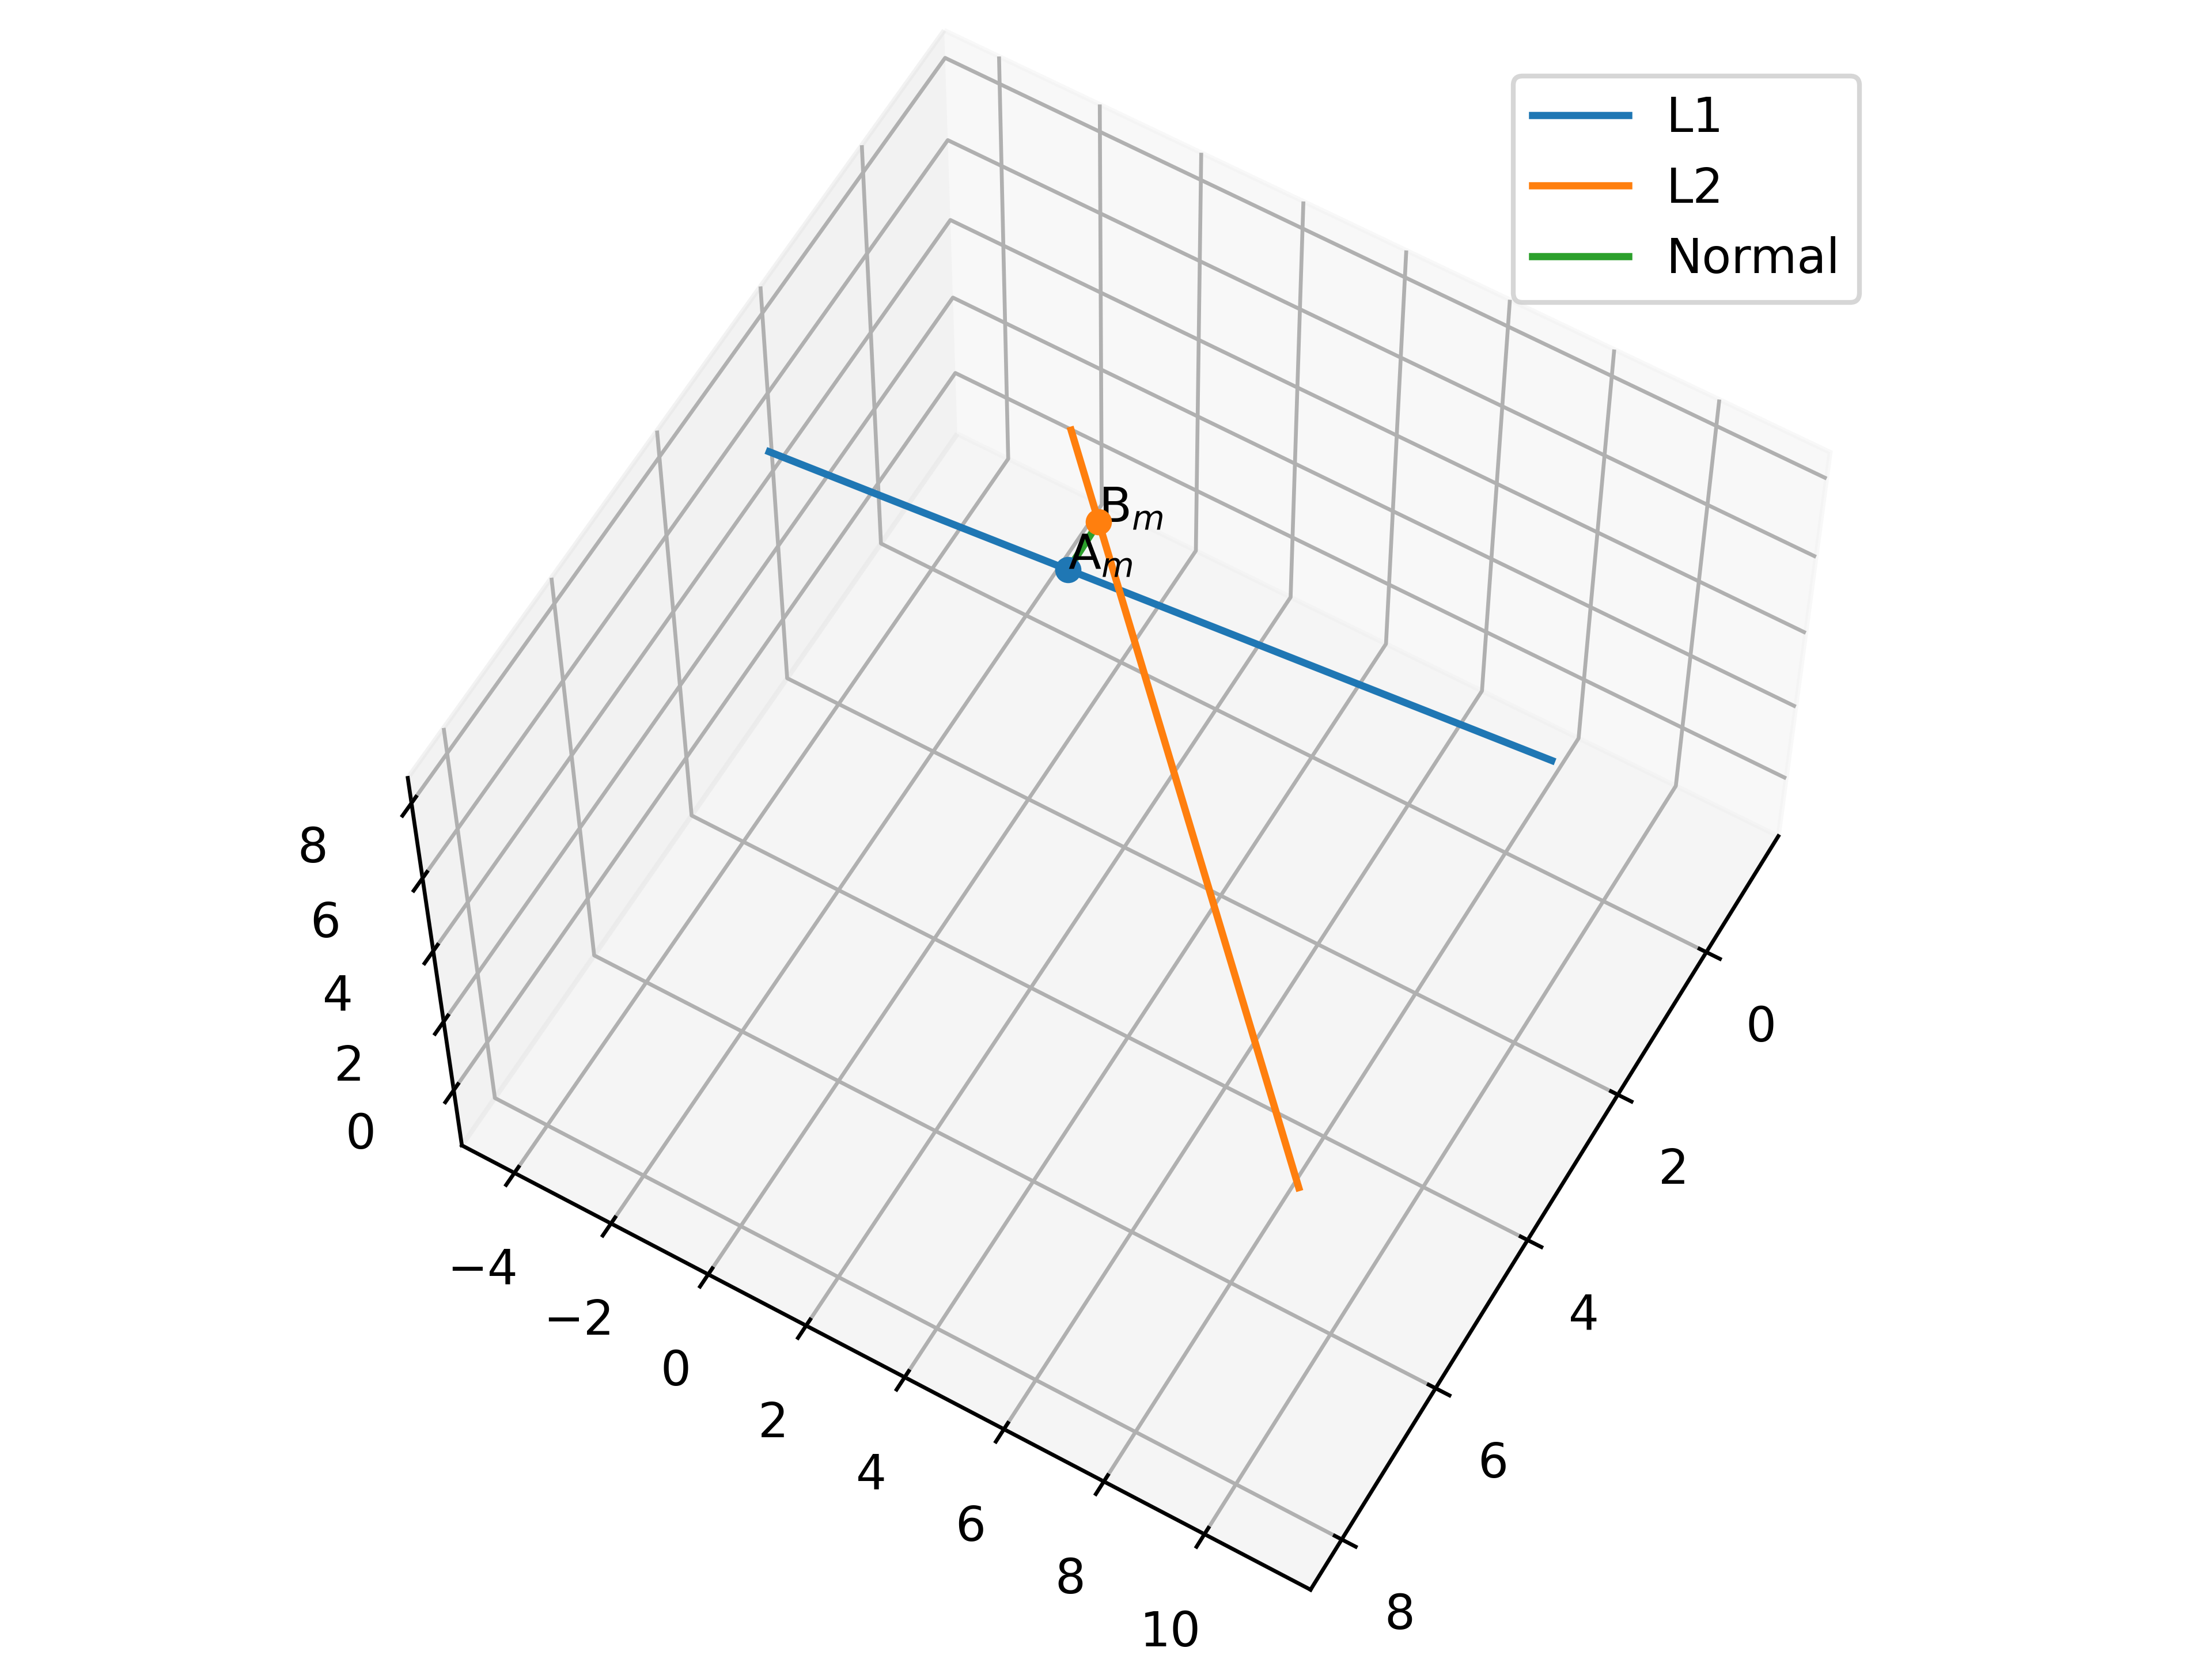
\includegraphics[width=0.75\columnwidth]{figs/skew_gd.png}
        \caption{Finding the shortest distance using gradient descent.}
        \label{fig:skew-gd}
    \end{figure}
\end{enumerate}
\end{document}
